\section{Set Theory}

This section introduces basic set notation, relations, and equivalence classes. The presentation follows the treatment of these foundations in \cite[Chapter 1, especially Section 1.6]{Berberian1998-qc}.

\subsection{Basic Set Notation}

\begin{definition}[Subset and equality]
Let $A$ and $B$ be sets. We say that $A$ is a subset of $B$, and write $A\subseteq B$, if every element of $A$ is also an element of $B$. The sets are equal if they have exactly the same elements; equivalently, $A=B$ if and only if $A\subseteq B$ and $B\subseteq A$.
\end{definition}

\begin{proposition}
For any sets $A$ and $B$, $A=B$ if and only if each is a subset of the other.
\end{proposition}

\begin{proof}
If $A=B$, then they have the same elements, so $A\subseteq B$ and $B\subseteq A$. Conversely, if both inclusions hold, an element belongs to $A$ exactly when it belongs to $B$. Thus the sets have the same elements and are equal.
\end{proof}

\begin{definition}[Set operations]
For sets $A$ and $B$, their union and intersection are
\[
 A\cup B=\{x:x\in A\text{ or }x\in B\},\qquad
 A\cap B=\{x:x\in A\text{ and }x\in B\}.
\]
Their difference is $A\setminus B=\{x\in A:x\notin B\}$. If a universal set $X$ is fixed and $A\subseteq X$, the complement of $A$ in $X$ is $X\setminus A$.
\end{definition}

\begin{definition}[Cartesian product]
For sets $X$ and $Y$, the Cartesian product is the set
\[
 X\times Y=\{(x,y):x\in X,\ y\in Y\}
\]
of ordered pairs.
\end{definition}

\subsection{Relations and Equivalence Relations}

\begin{definition}[Relation]
A relation from a set $X$ to a set $Y$ is a subset $R\subseteq X\times Y$. A relation in $X$ is a relation from $X$ to itself. We write $x\,R\,y$ when $(x,y)\in R$.
\end{definition}

\begin{definition}[Equivalence relation]
A relation $\sim$ in a set $X$ is an equivalence relation if, for all $x,y,z\in X$, it is:
\begin{enumerate}
    \item reflexive: $x\sim x$;
    \item symmetric: if $x\sim y$, then $y\sim x$;
    \item transitive: if $x\sim y$ and $y\sim z$, then $x\sim z$.
\end{enumerate}
\end{definition}

\begin{example}[Equality of function values]
Let $f:X\to Y$ be a function. Define $x\sim y$ when $f(x)=f(y)$. This is an equivalence relation: equality is reflexive, symmetric, and transitive, so the same three properties hold for $\sim$.
\end{example}

\subsection{Equivalence Classes and Quotient Sets}

\begin{definition}[Equivalence class]
If $\sim$ is an equivalence relation on $X$ and $x\in X$, the equivalence class of $x$ is
\[
 [x]=\{y\in X:y\sim x\}.
\]
The quotient set is the set of all equivalence classes,
\[
 X/{\sim}=\{[x]:x\in X\}.
\]
\end{definition}

\begin{theorem}[Equivalence classes partition a set]
Let $\sim$ be an equivalence relation on $X$. Every element of $X$ belongs to an equivalence class, and any two equivalence classes are either equal or disjoint.
\end{theorem}

\begin{proof}
Reflexivity gives $x\sim x$, so $x\in[x]$ for each $x\in X$. Now suppose $[x]\cap[y]\ne\varnothing$ and choose $z\in[x]\cap[y]$. Then $z\sim x$ and $z\sim y$. By symmetry and transitivity, $x\sim y$. If $t\in[x]$, then $t\sim x$ and $x\sim y$, so $t\sim y$ and $t\in[y]$. Thus $[x]\subseteq[y]$; the same argument with $x$ and $y$ interchanged gives $[y]\subseteq[x]$. Hence $[x]=[y]$.
\end{proof}

\begin{corollary}
Two elements $x,y\in X$ are equivalent if and only if their equivalence classes are equal.
\end{corollary}

\begin{proof}
If $x\sim y$, transitivity and symmetry show that an element belongs to $[x]$ exactly when it belongs to $[y]$, so $[x]=[y]$. Conversely, if $[x]=[y]$, then $x\in[x]=[y]$, which means $x\sim y$.
\end{proof}

\begin{example}[Integers modulo $m$]
Fix a positive integer $m$. On $\mathbb{Z}$, define $a\sim b$ if $m$ divides $a-b$. This is an equivalence relation: $m$ divides $a-a=0$; divisibility of $a-b$ implies divisibility of $b-a$; and if $m$ divides both $a-b$ and $b-c$, it divides their sum $a-c$. Its equivalence classes collect the integers with the same remainder upon division by $m$.
\end{example}
Taking $m=3$ gives a concrete partition of $\mathbb{Z}$. Each row below displays representative integers from one equivalence class; the ellipses indicate that each class continues indefinitely in both directions.
\[
 [r]_3=\{r+3k:k\in\mathbb{Z}\},\qquad r\in\{0,1,2\},
 \qquad
 \mathbb{Z}=[0]_3\,\dot\cup\,[1]_3\,\dot\cup\,[2]_3.
\]

\begin{figure}[htbp]
\centering
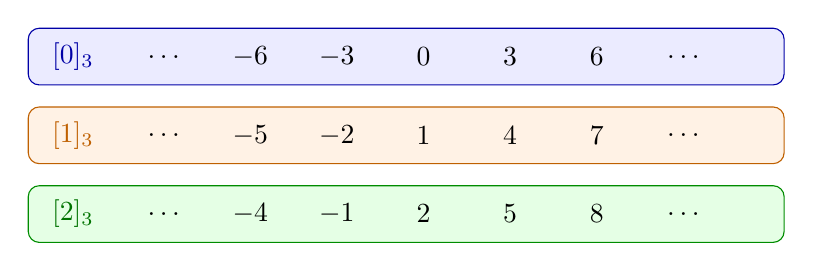
\begin{tikzpicture}[x=1.1cm,y=1cm]
    \node[draw=blue!65!black,fill=blue!8,rounded corners,minimum width=9.6cm,minimum height=0.72cm,inner sep=2pt] at (4.8,2) {};
    \node[draw=orange!75!black,fill=orange!10,rounded corners,minimum width=9.6cm,minimum height=0.72cm,inner sep=2pt] at (4.8,1) {};
    \node[draw=green!55!black,fill=green!10,rounded corners,minimum width=9.6cm,minimum height=0.72cm,inner sep=2pt] at (4.8,0) {};

    \node[anchor=west,text=blue!65!black,font=\bfseries] at (0.6,2) {$[0]_3$};
    \node[anchor=west,text=orange!75!black,font=\bfseries] at (0.6,1) {$[1]_3$};
    \node[anchor=west,text=green!45!black,font=\bfseries] at (0.6,0) {$[2]_3$};

    \foreach \x/\value in {2.0/{\ldots},3.0/{-6},4.0/{-3},5.0/{0},6.0/{3},7.0/{6},8.0/{\ldots}} {
        \node at (\x,2) {$\value$};
    }
    \foreach \x/\value in {2.0/{\ldots},3.0/{-5},4.0/{-2},5.0/{1},6.0/{4},7.0/{7},8.0/{\ldots}} {
        \node at (\x,1) {$\value$};
    }
    \foreach \x/\value in {2.0/{\ldots},3.0/{-4},4.0/{-1},5.0/{2},6.0/{5},7.0/{8},8.0/{\ldots}} {
        \node at (\x,0) {$\value$};
    }
\end{tikzpicture}
\caption{The equivalence classes of integers modulo $3$. Each row is one class; distinct rows are disjoint and together contain all integers.}
\label{fig:equivalence-classes-mod-3}
\end{figure}